% Fig. 5 assembled from its panels; run from the directory that holds them.
\documentclass[tikz,border=1mm]{standalone}
\usepackage{graphicx,xcolor}
\usetikzlibrary{fit,positioning,calc,backgrounds,arrows.meta}
\usepackage[T1]{fontenc}
\usepackage{DejaVuSans}\renewcommand{\familydefault}{\sfdefault}
\graphicspath{{./}}
\definecolor{rose}{HTML}{D40054}
\definecolor{teal}{HTML}{006680}
\definecolor{inkgray}{HTML}{6B6B6B}
\newcommand{\pnl}[5]{% name, x, y (mm, top-left), file, LETTER
  \node[anchor=north west,inner sep=0] (#1) at (#2mm,#3mm) {\includegraphics{#4}};
  \node[anchor=north west,font=\bfseries\fontsize{8}{8}\selectfont,inner sep=1pt] at (#1.north west) {#5};}
\newcommand{\blockbox}[5]{% fit list, edge colour, title, inner xsep, inner ysep  (outline only)
  \begin{scope}[on background layer]
    \node[draw=#2,line width=1.4pt,draw opacity=0.5,rounded corners=2mm,fill=none,inner xsep=#4,inner ysep=#5,fit=#1] (box) {};
  \end{scope}
  \node[anchor=center,fill=#2,text=white,font=\bfseries\fontsize{7}{7}\selectfont,rounded corners=1.2mm,inner xsep=2.5mm,inner ysep=1mm] at (box.north) {#3};}
\begin{document}
\begin{tikzpicture}[x=1mm,y=1mm]
\pnl{b}{0}{0}{hhe_main_b.png}{a}
\node[anchor=north west,inner sep=0,draw=inkgray,line width=0.3pt] (s1) at (6mm,-31.5mm) {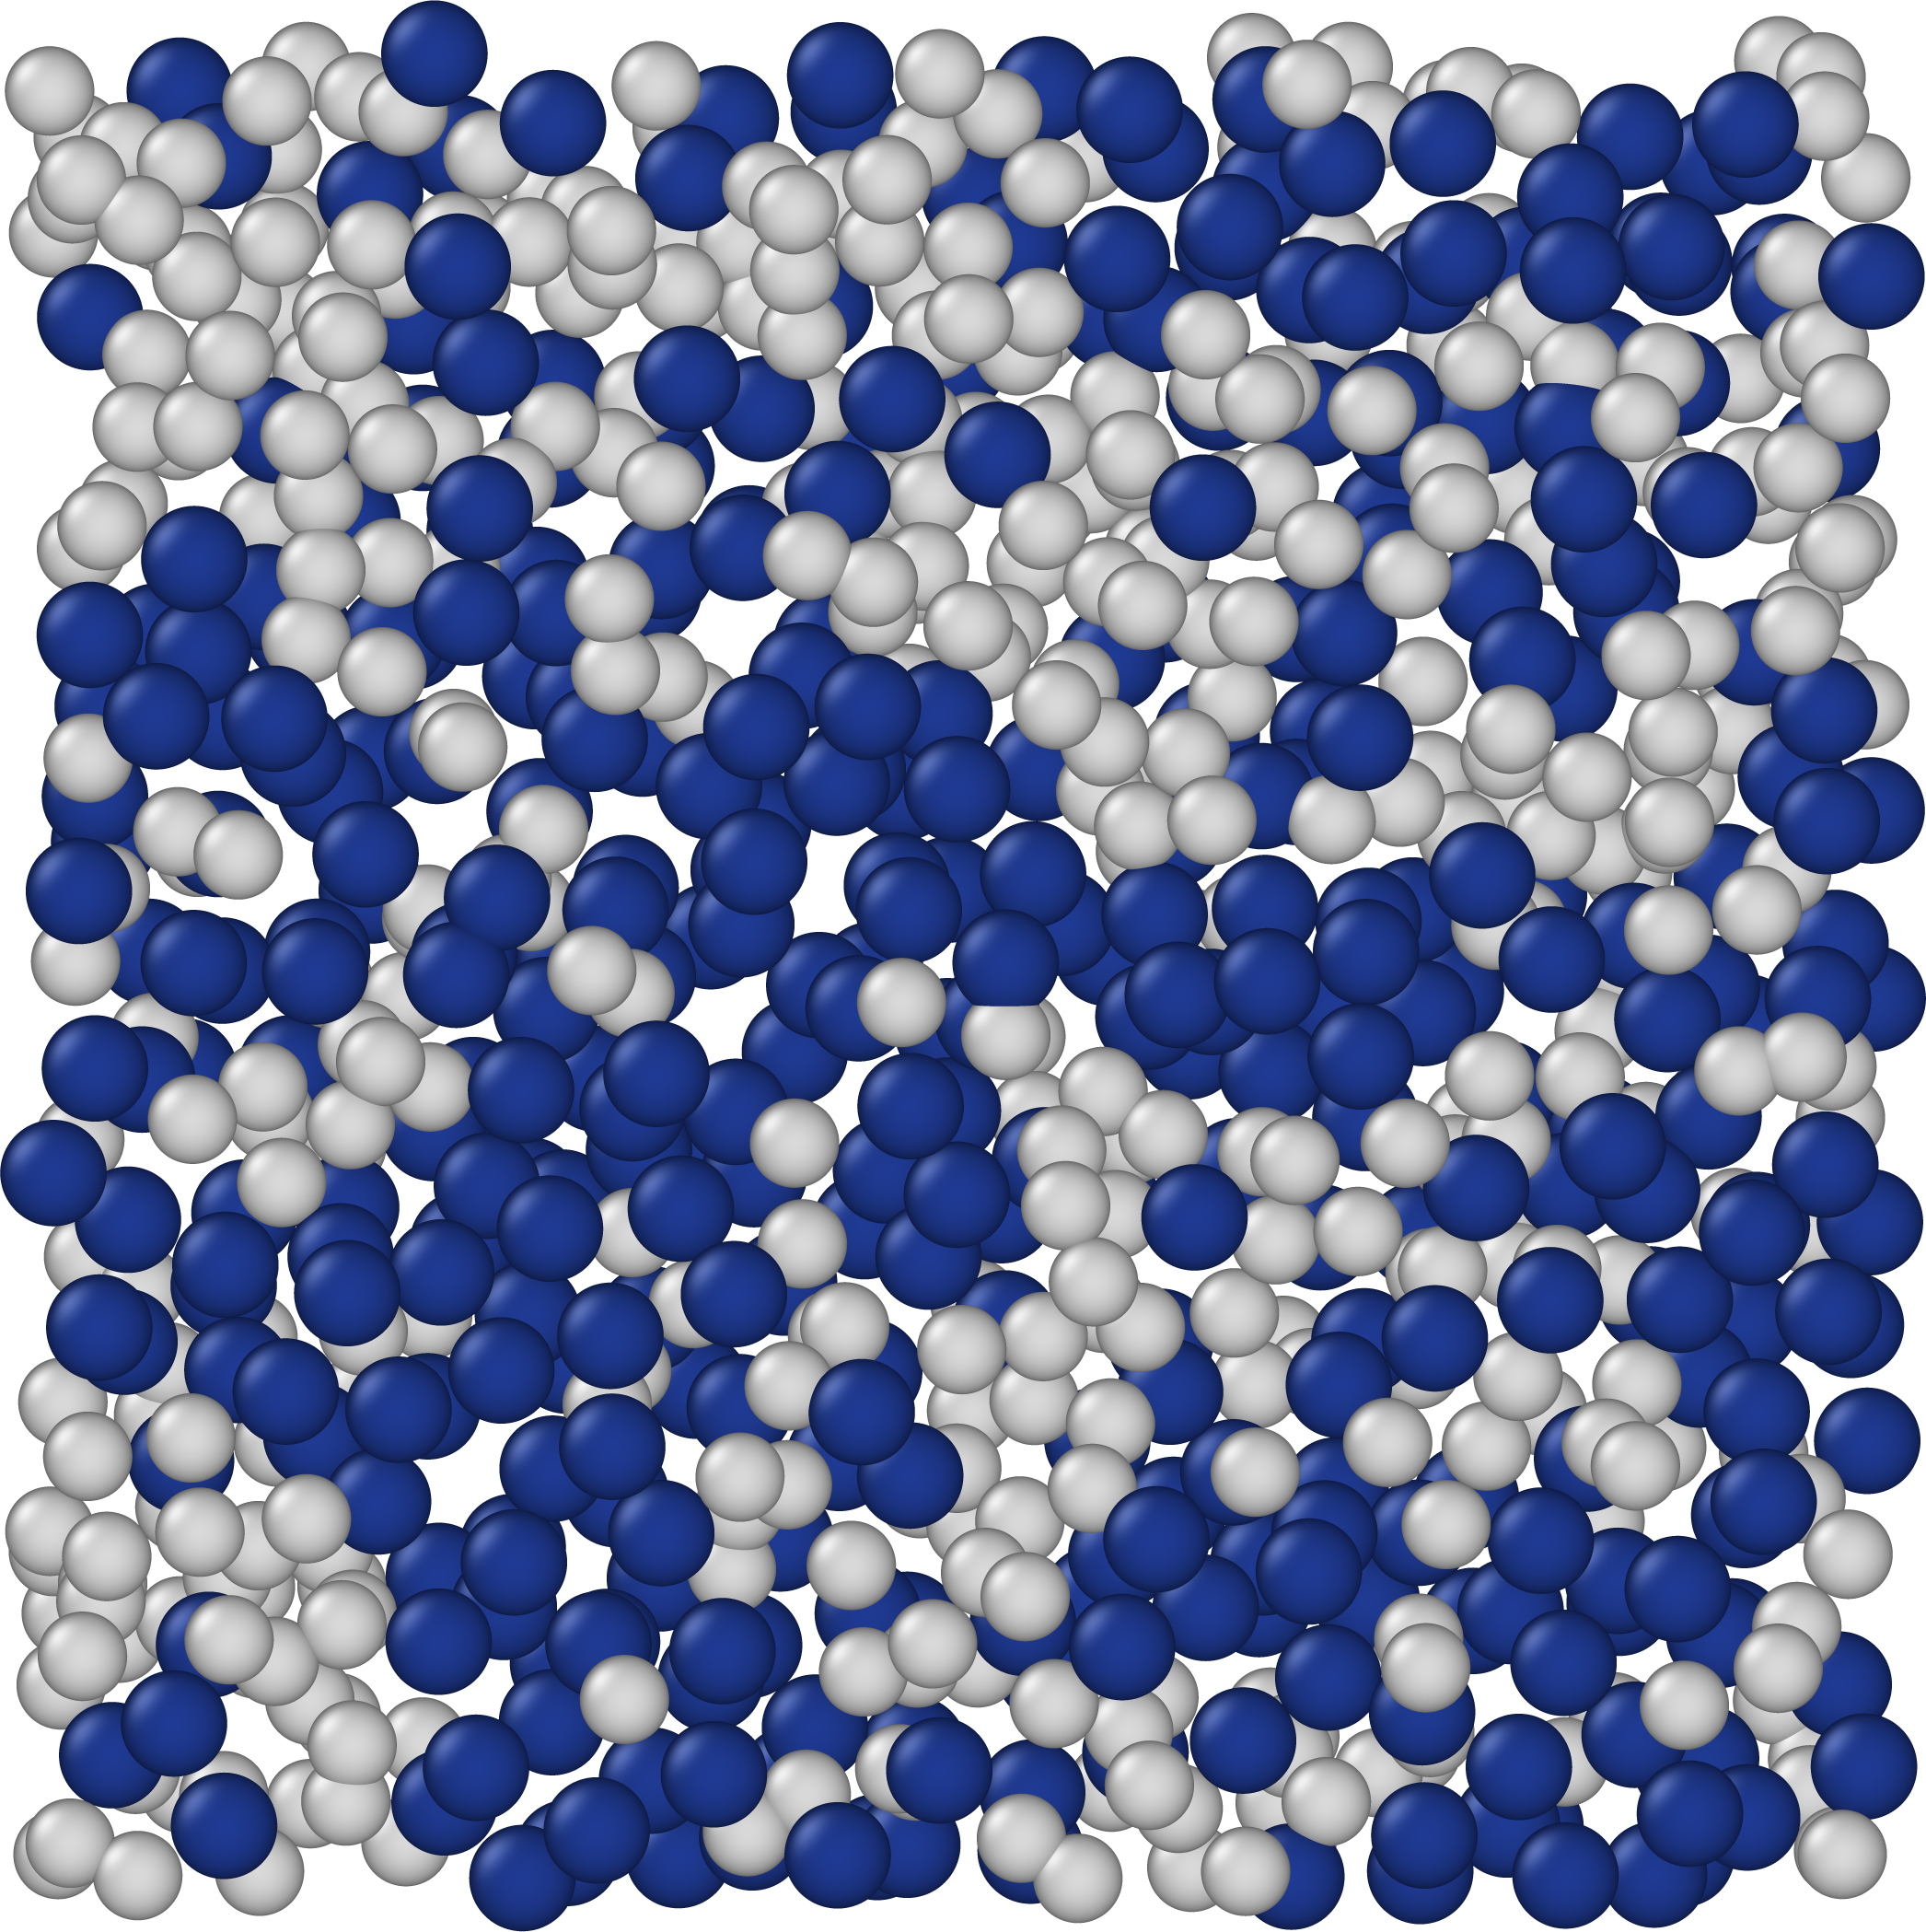
\includegraphics[width=16mm]{md_snapshot_T10000_slab.png}};
\node[anchor=north west,inner sep=0,draw=inkgray,line width=0.3pt] (s2) at (28mm,-31.5mm) {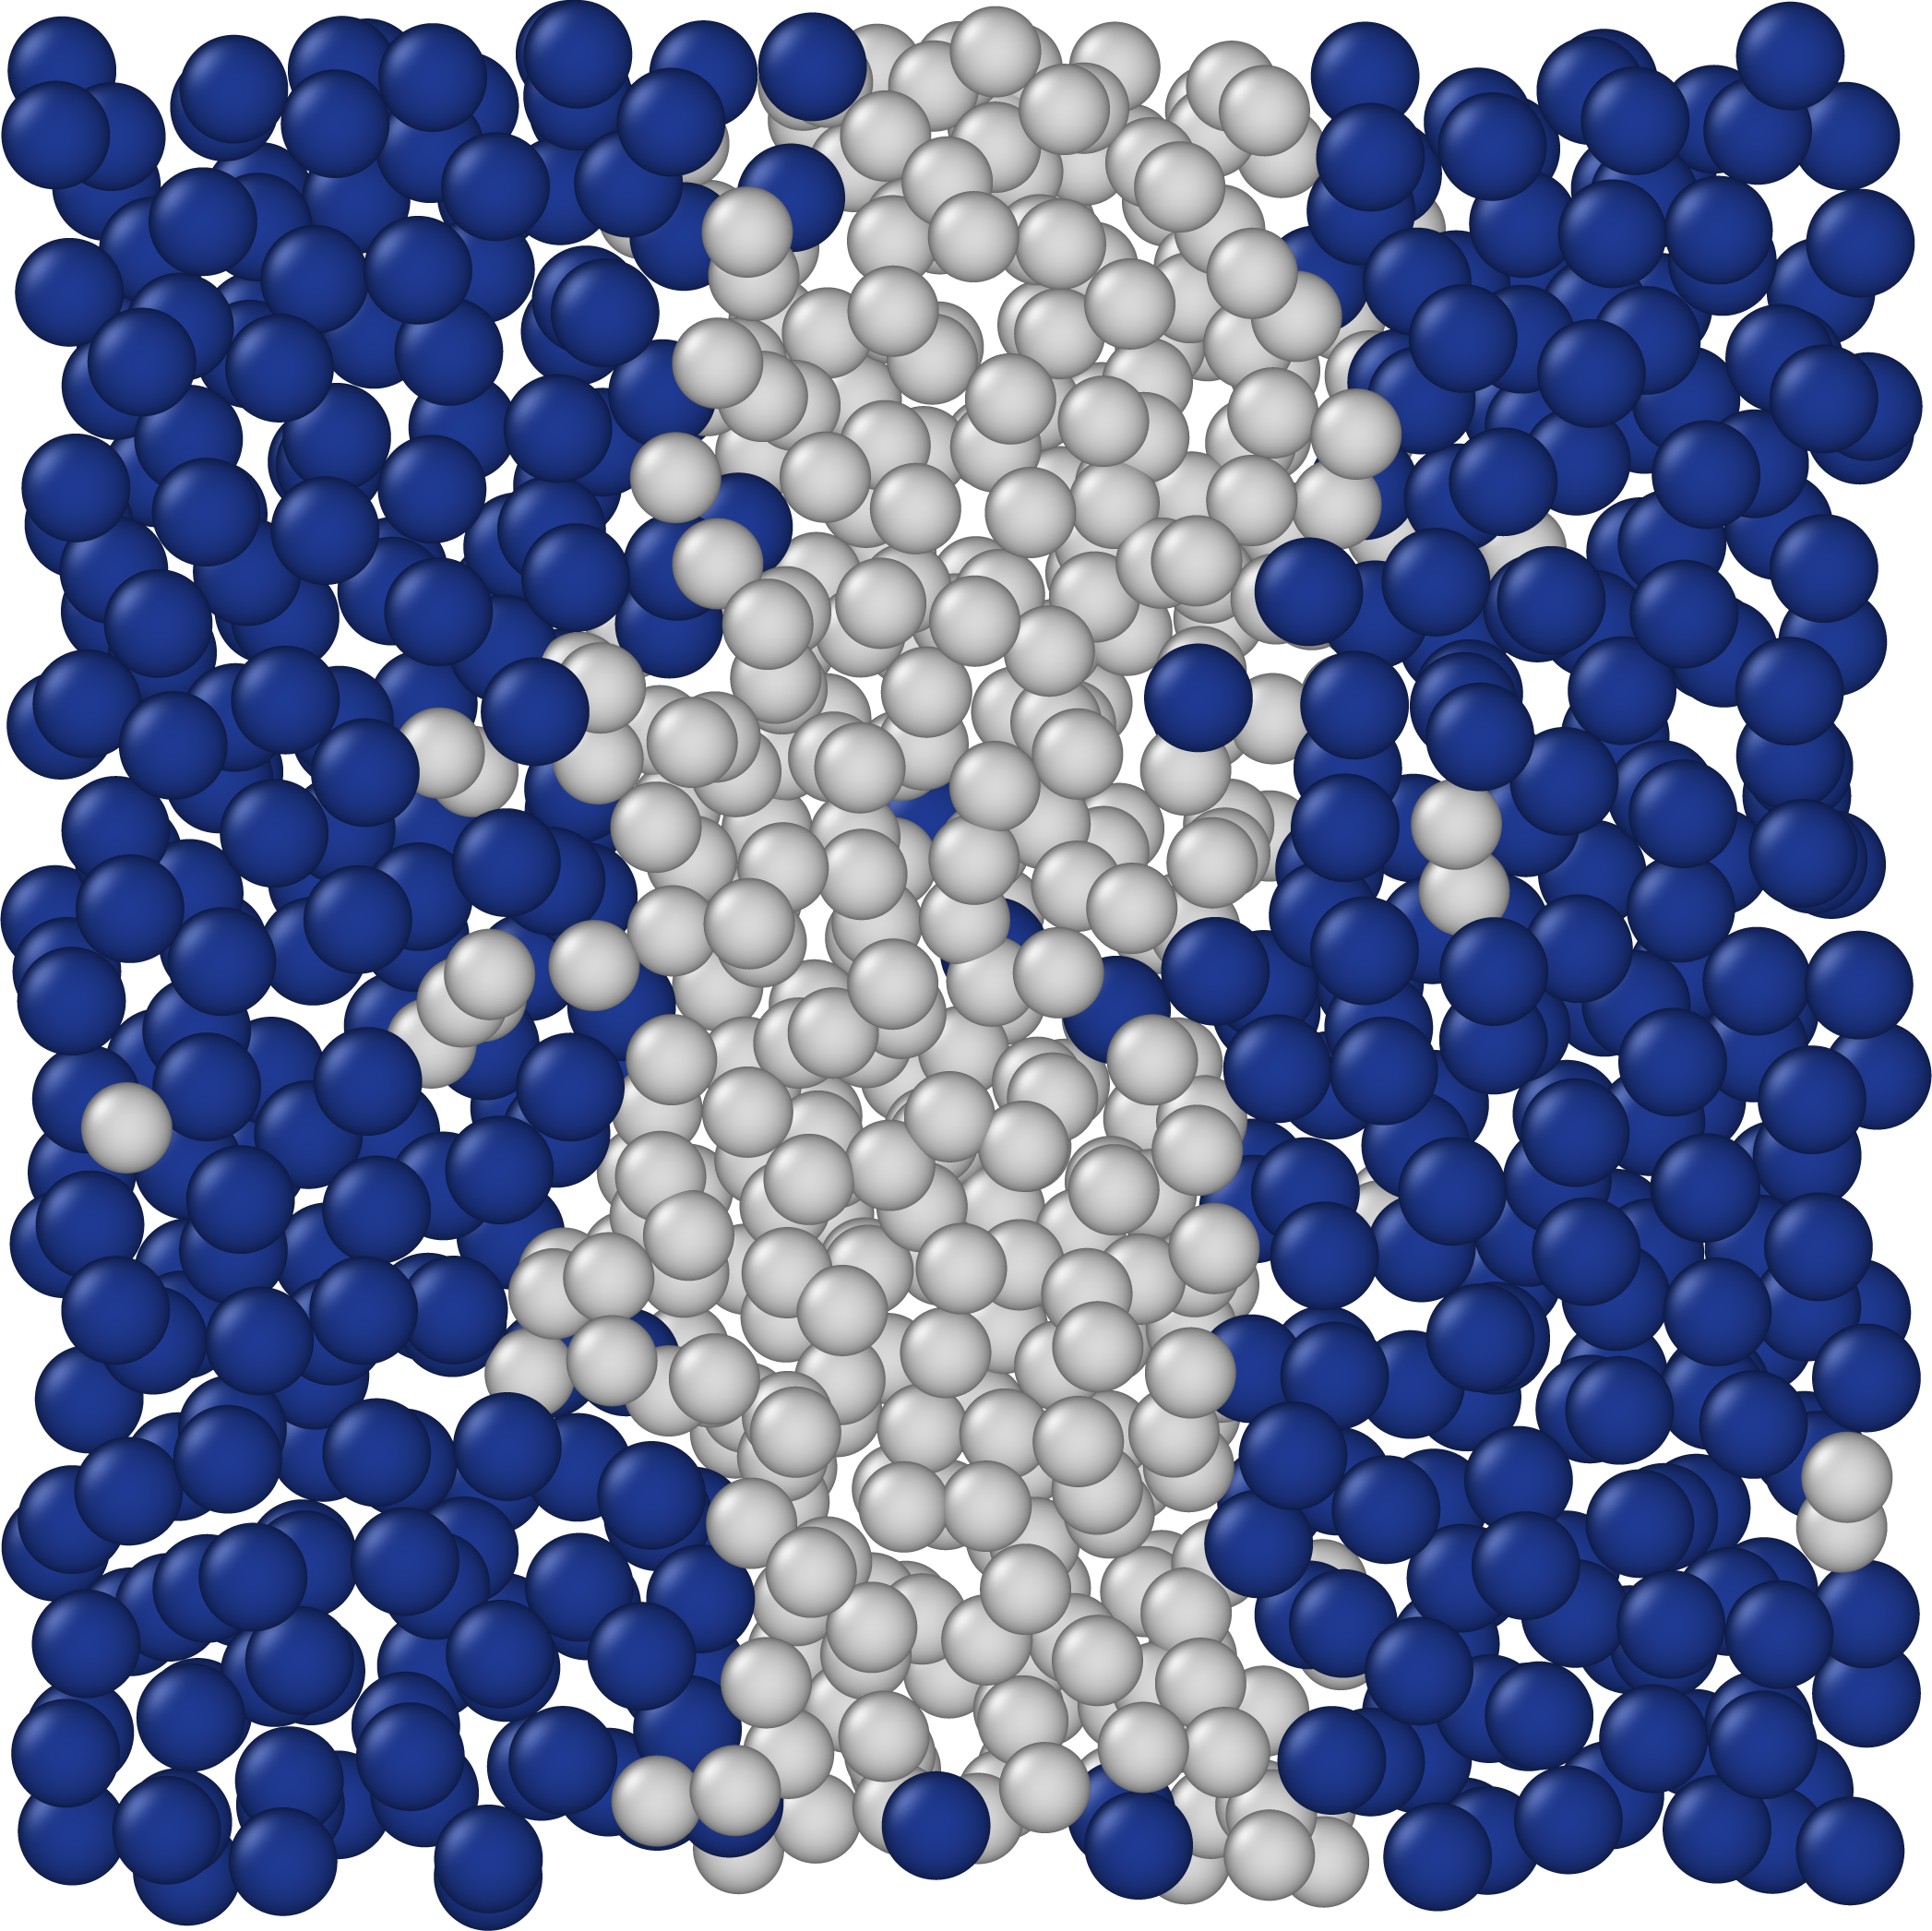
\includegraphics[width=16mm]{md_snapshot_T05000_slab.png}};
\coordinate (mix) at ($(b.north west)+(11.5mm,-8.5mm)$);
\coordinate (dem) at ($(b.north west)+(24mm,-20.5mm)$);
\fill[black!45] (mix) circle (0.4mm);
\fill[black!45] (dem) circle (0.4mm);
\draw[-{Stealth[length=1.2mm]},line width=0.4pt,black!45] (mix) to[out=-100,in=90] ($(s1.north west)+(1.5mm,0)$);
\draw[-{Stealth[length=1.2mm]},line width=0.4pt,black!45] (dem) to[bend left=10] (s2.north);
\pnl{c}{0}{-51}{hhe_main_c.pdf}{b}
\pnl{a}{57}{1.5}{hhe_main_a.pdf}{c}
\pnl{l}{84.5}{1.5}{hhe_main_lit.pdf}{d}
\pnl{d}{131}{1.5}{hhe_main_d.pdf}{e}
\node[anchor=north west,inner sep=0] (e) at (57mm,-51mm) {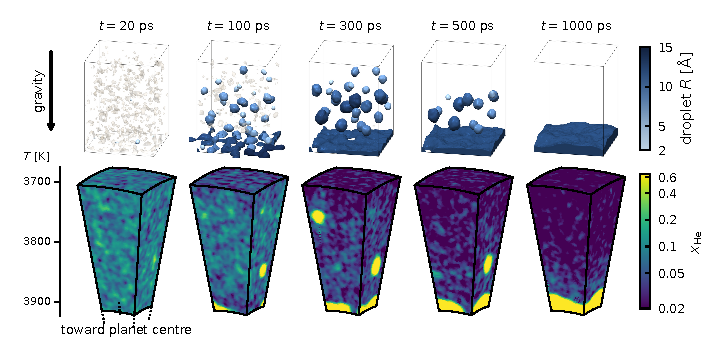
\includegraphics{hhe_main_fg.pdf}};
\node[anchor=north west,font=\bfseries\fontsize{8}{8}\selectfont,inner sep=1pt] at (e.north west) {f};
\node[anchor=north west,font=\bfseries\fontsize{8}{8}\selectfont,inner sep=1pt] at ($(e.north west)+(0mm,-26.0mm)$) {g};
\coordinate (f) at (e.south east);
\blockbox{(b)(c)(s1)(s2)}{rose}{Phase diagram}{3.5mm}{3.5mm}
\blockbox{(a)(l)(d)}{inkgray}{Helium rain in gas giants}{3.5mm}{2mm}
\blockbox{(e)(f)}{teal}{Dynamics}{3.5mm}{3.5mm}
\end{tikzpicture}
\end{document}
